
\problemname{Flyttkartonger}

Du har just hjälpt en kompis att flytta, men tyvärr har du fastnat i
fel ände av en smal korridor full med flyttkartonger. Korridoren
består av $N$ staplar av flyttkartonger, där stapel nummer $i$
innehåller $a_i$ kartonger. Alla kartonger är lika stora.

Det enda sättet att ta sig ut är att gå ovanpå staplarna från stapel
$1$ till stapel $N$. Om man befinner sig på en stapel kan man gå till
en närliggande stapel, men bara om den inte är högre än den man står
på. Om stapeln man står är minst två kartonger högre än en närliggande
stapel kan man dessutom knuffa ner den översta kartongen från stapeln
man står på till den närliggande stapeln. Detta kan upprepas hur många
gånger som helst. 

Du befinner dig just nu på stapel $1$. Tyvärr kanske det är omöjligt
för dig att komma till stapel $N$. Men som tur är får du lägga till
valfritt antal {\em extra} kartonger till stapel $1$ innan du börjar gå. Skriv ett program som
beräknar hur många extra kartonger du behöver lägga till för att kunna
ta dig till stapel $N$.

\begin{figure}[!h]
\begin{center}
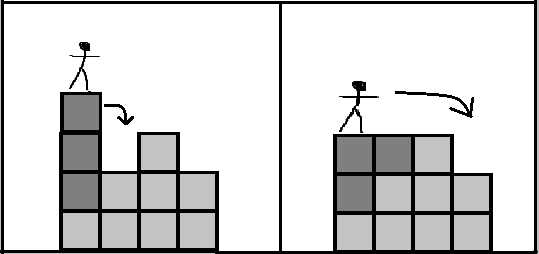
\includegraphics[width=0.9\textwidth]{kartongbild2.png}
\end{center}
\caption{Bilden visar exempel $1$. De mörkgrå kartongerna är extrakartonger. Strategin är alltså att knuffa ner den översta extrakartongen till stapel $2$. Därefter kan man gå raka vägen till stapel $4$. Det hade inte hade fungerat med färre än $3$ extrakartonger.}
\end{figure}

\section*{Indata}
På första raden står ett heltal $N$, antalet staplar. På andra raden står $N$ heltal $a_i$, antalet kartonger i varje stapel. 

\section*{Utdata}
Skriv ut ett heltal: det minsta antalet extra flyttkartonger som behöver läggas till.


\section*{Poängsättning}
Din lösning kommer att testas på en mängd testfallsgrupper.
För att få poäng för en grupp så måste du klara alla testfall i gruppen.

\noindent
\begin{tabular}{| l | l | l |}
  \hline
  Grupp & Poängvärde & Gränser \\ \hline
  $1$   & $20$       & $N=3, 1 \leq a_i \leq 20$ \\ \hline
  $2$   & $20$       & $3 \leq N \leq 5, 1 \leq a_i \leq 100$ \\ \hline
  $3$   & $20$       & $5 \leq N \leq 10, 1 \leq a_i \leq 1\,000$ \\ \hline
  $4$   & $40$       & $10 \leq N \leq 20, 1 \leq a_i \leq 3\,000$ \\ \hline
\end{tabular}
